% !TEX root = ReviewDraft.tex





\section{Entropy of an evaporating black hole}



In this section, we will see how to apply the fine-grained entropy  formula \eqref{RT} to all stages of the evaporating black hole.  










	Let us first compute the entropy after the black hole forms but before any Hawking radiation has a chance to escape the black hole region.
	In this case, there are no extremal surfaces encountered by deforming $X$ inwards, and we are forced to shrink it all the way down to zero size.  See figure \ref{CollapseRT}. The area term vanishes, so the fine-grained entropy is just the entropy of the matter enclosed by the cutoff surface. 
	Note that this calculation is sensitive to the geometry in the interior of the black hole.  	This means that the entropy at the initial stage will vanish,  assuming that the collapsing shell was in a pure state.\footnote{   We are neglecting the contribution from the  entanglement of the fields near the cutoff surface. We are taking this contribution to be time independent, and we implicitly subtract it in our discussion.}   If we ignore the effects of Hawking radiation, this fine-grained entropy is invariant under time evolution. This is in contrast with the area of the horizon, which starts out being zero at $r=0$ and then grows to $4\pi r_s^2$ after the black hole forms. 
	





Once the black hole starts evaporating and the outgoing Hawking quanta escape the black hole region, the von Neumann entropy of this region will no longer be zero due to the entanglement between the interior Hawking quanta and those that escaped. As shown in figure \ref{nicesliceentropy}, this entropy continues to grow as the black hole evaporates due to the pile up of the mixed interior modes. This growth of  entropy precisely parallels that of the outgoing Hawking radiation, and seems to support the idea that the black hole can have arbitrarily larger entropy than its Area$/4G_N$, inconsistent with the central dogma. 

\begin{figure}[h]
\begin{center}
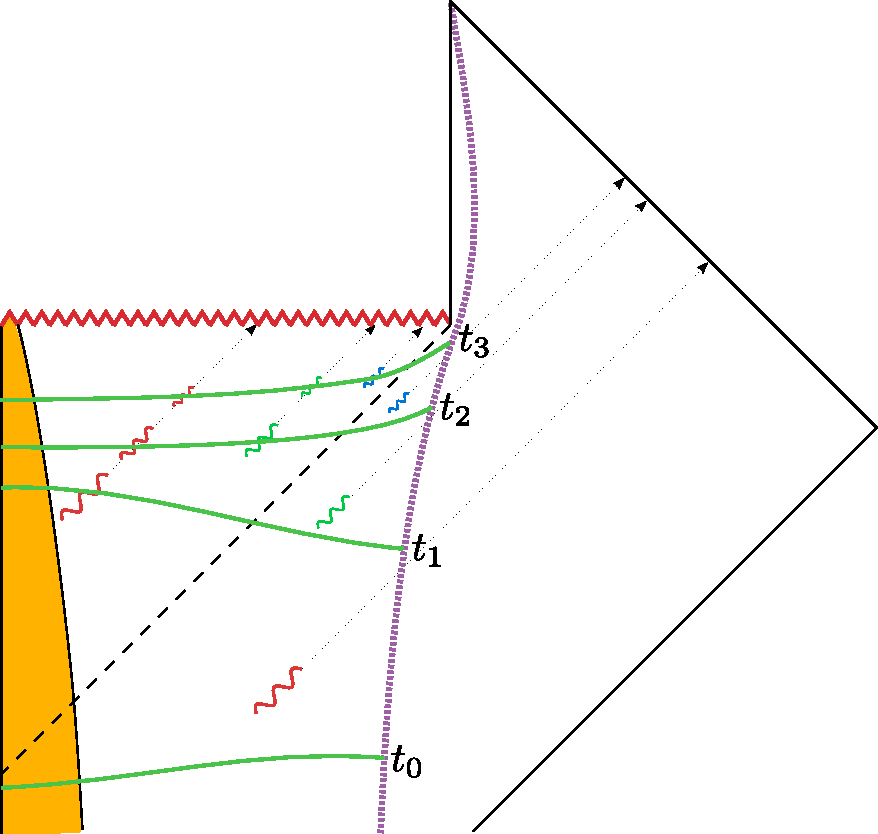
\includegraphics[scale=0.39]{figures/nicesliceentropy.pdf}
 \ \ \ \ \ \ 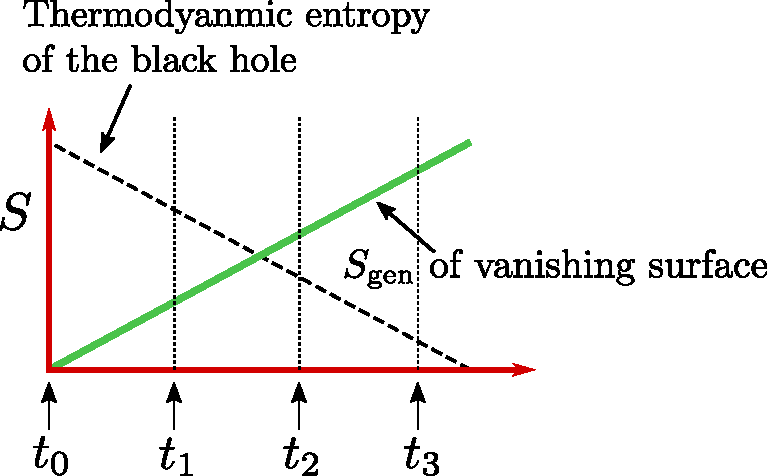
\includegraphics[scale=0.56]{figures/trivialcurve.pdf}
\caption{As more outgoing Hawking quanta escape the black hole region, its entropy grows due to the pile up of interior Hawking quanta. Modes of like colors are entangled with one another. On the right is a plot comparing this growing entropy to the decreasing thermodynamic entropy of the black hole. }
\label{nicesliceentropy}
\end{center}
\end{figure}

\begin{figure}[t]
\begin{center}
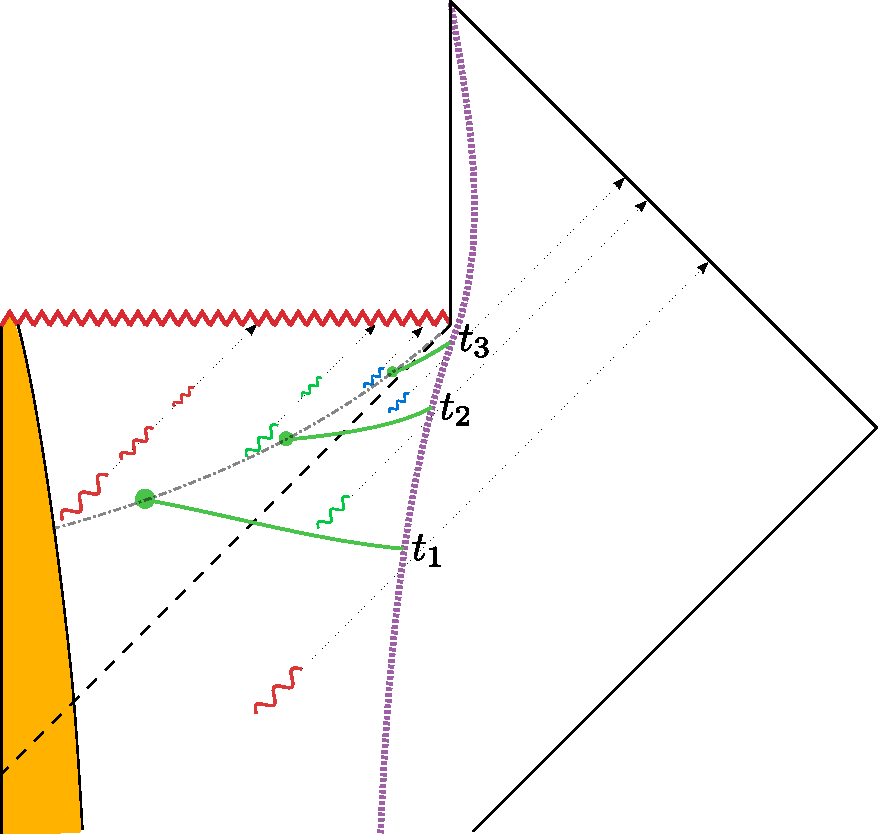
\includegraphics[scale=0.39]{figures/nontrivialsurface.pdf}
 \ \ \ \ \ \ 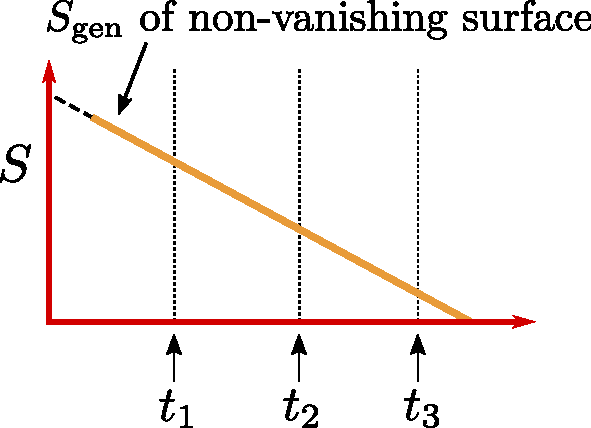
\includegraphics[scale=0.56]{figures/nontrivialcurve.pdf}
\caption{When the non-vanishing extremal surface first appears, it lies inside the black hole near the event horizon. For different times on the cutoff surface, it is a different surface which moves along a spacelike direction up the horizon. This gives a decreasing generalized entropy since the black hole area is shrinking.}
\label{nontrivialsurface}
\end{center}
\end{figure}

The story is not yet complete since there is also a non-vanishing extremal surface that appears  shortly after the Hawking radiation starts escaping the black hole region. The precise location of this surface depends on how much radiation has escaped, and hence on the time $t$ along the cutoff surface when we decide to compute the entropy. 
It turns out that the surface lies close to the event horizon. 
Its location along the horizon is determined as follows. We go back along the cutoff surface by a time of order $r_s \log S_{BH}$ and we shoot an ingoing light ray. Then the surface is located close to the point where this light ray intersects the horizon. Note that $r_s$, and also $r_s \log S_{BH}$, are times which are short compared to the evaporation time, $r_s S_{BH}$. The time scale $r_s \log S_{BH}$ is called ``the scrambling time'' and it   has an interesting significance that we will not discuss in this review, see e.g. \cite{Hayden:2007cs,Sekino:2008he}. 
This is shown in figure \ref{nontrivialsurface}. The generalized entropy  now has an area term as well as the von Neumann entropy of quantum fields, $\Ssemi$. %Since the `outside' region for this surface no longer captures a lot of Hawking quanta, 
This quantum field theory entropy is relatively small because it does not capture many Hawking quanta and thus the  entropy is dominated by the area term
%  Therefore, it is well approximated by the area of the horizon
\begin{align}
S_\mathrm{gen} \approx {\mathrm{Horizon \ Area}(t)  \over 4 G_N} \,.
\end{align}
This generalized entropy follows closely the evolution of the thermodynamic entropy of the black hole. Since the area of the black hole decreases as it evaporates, this extremal surface gives a decreasing generalized entropy. 


The complete proof for the existence of this surface would be to show that the change of area of $X$ under a small deformation in any direction perfectly balances the change in the von Neumann entropy  $\Ssemi$. We give some intuition for this procedure by extremizing along the ingoing null direction. The key point is that, while the area of $X$ is monotonically decreasing along this direction,  the entropy  $\Ssemi$ is not. To see this, imagine starting with $X$ right on the horizon and analyze the entanglement pattern across the surface as it is moved inwards. As the surface is moved inwards, the entropy $\Ssemi$   decreases as the newly included interior Hawking modes  purify the outgoing quanta already included in the region `outside.' Once all of those outgoing quanta have been purified, moving the surface inward further would start including modes entangled with outgoing quanta outside the black hole region thereby increasing $\Ssemi$. It is in this regime that changes in the area and entropy can exactly balance each other out. For the precise equations see \cite{Almheiri:2019psf,Penington:2019npb}. 
 

\begin{figure}[t]
\begin{center}
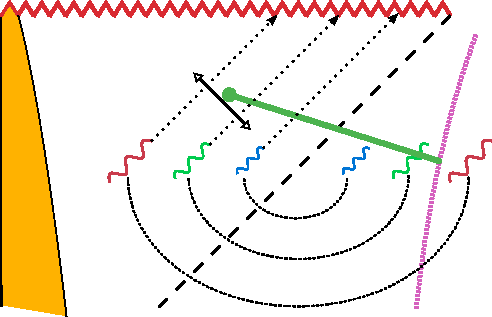
\includegraphics[scale=.5]{figures/simpleextremization}
\caption{$S_\mathrm{semi\text{-} cl}$ begins to increase when going inwards along the ingoing null coordinate once all the outgoing Hawking quanta in the black hole region are purified by the newly included interior modes. This allows for an extremum along this direction since the area of the surface shrinks.   }
\label{simpleextremization}
\end{center}
\end{figure}





Full application of the entropy formula \eqref{RT} requires taking the minimum of the generalized entropy over all available extremal surfaces. We found two such surfaces: a growing contribution from the vanishing    surface and a decreasing one from the non-vanishing  surface just behind the event horizon. At very early times, only the vanishing surface exists, giving a contribution which starts at zero and grows monotonically until the black hole evaporates away. Some short time after the black hole forms, the non-vanishing surface is created and it starts with a large value given by the current area of the black hole, and decreases as the black hole shrinks. Therefore, the vanishing surface initially captures the true fine-grained entropy of the black hole, up until  the non-vanishing surface contribution becomes smaller and starts to represent the true fine-grained entropy. In this way, by transitioning between these two contributions, the entropy of the black hole closely follows the Page curve indicative of unitary black hole evaporation, see figure \ref{both}. 


\begin{figure}[t]
\begin{center}
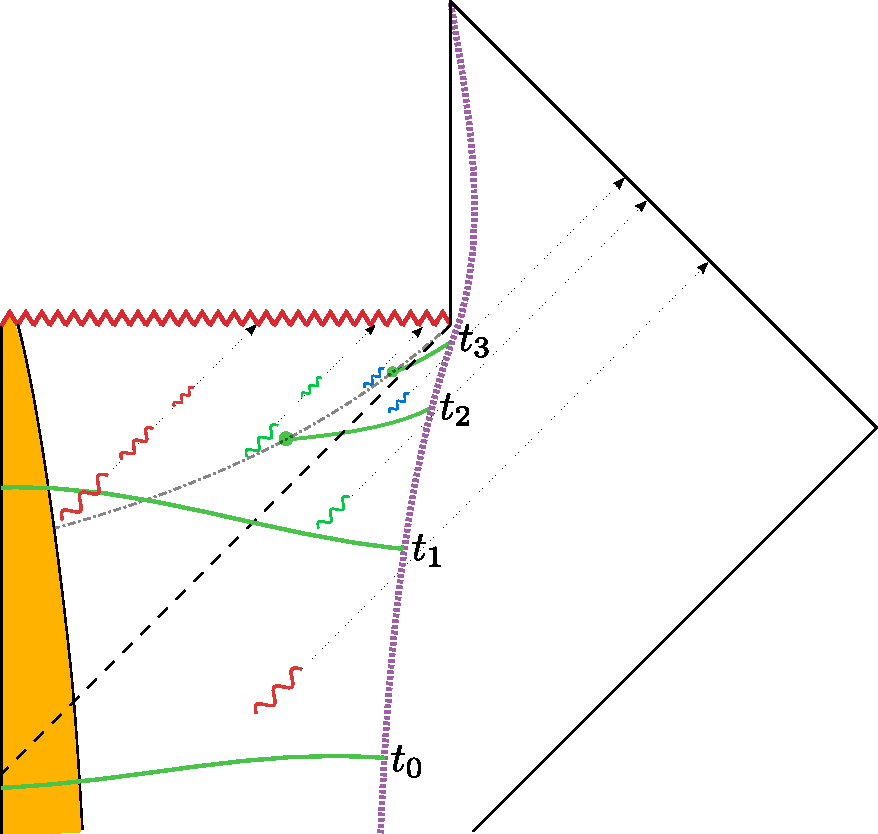
\includegraphics[scale=0.39]{figures/surfacetransition.pdf}
 \ \ \ \ \ \ 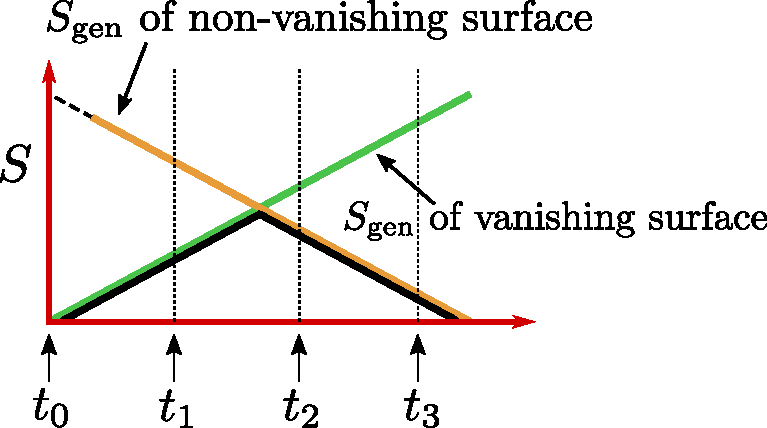
\includegraphics[scale=0.56]{figures/bothcurves.pdf}
\caption{The Page curve for the fine-grained entropy  of the black hole  (shown in black) is captured by the transition between a growing contribution from the trivial surface and a decreasing contribution from a non-trivial surface near the black hole horizon.}
\label{both}
\end{center}
\end{figure}





 
  

